\documentclass[11pt,a4paper]{article}
\usepackage[utf8]{inputenc}
\usepackage[T1]{fontenc}
\usepackage[brazil]{babel}
\usepackage{lmodern}
\usepackage{amsmath,amssymb,amsthm}
\usepackage{graphicx}
\usepackage{booktabs}
\usepackage[margin=2.5cm]{geometry}
\usepackage[colorlinks=true,linkcolor=blue!50!black,citecolor=blue!50!black,urlcolor=blue!50!black]{hyperref}
\usepackage{stmaryrd}
\usepackage{xcolor}

\numberwithin{equation}{section}
\newtheorem{teorema}{Teorema}[section]
\newtheorem{proposicao}[teorema]{Proposição}
\newtheorem{corolario}[teorema]{Corolário}
\newtheorem{lema}[teorema]{Lema}
\theoremstyle{definition}
\newtheorem{hipotese}{Hipótese}
\renewcommand{\thehipotese}{(A\arabic{hipotese})}
\newtheorem{definicao}[teorema]{Definição}
\theoremstyle{remark}
\newtheorem{observacao}[teorema]{Observação}

\newcommand{\R}{\mathbb{R}}
\newcommand{\E}{\mathcal{E}}
\newcommand{\jump}[1]{\llbracket #1 \rrbracket}
\newcommand{\dd}{\,\mathrm{d}}
\newcommand{\Hs}{H^{*}}
\newcommand{\Ps}{P^{*}}

\title{O paradoxo dos pesticidas com difusão espacial e\\ aplicação de suporte compacto\\[4pt]
\large Uma generalização do modelo de Li \& Yang (2015)}
\author{}
\date{Outubro de 2026}

\begin{document}
\maketitle

\begin{abstract}
Li e Yang \cite{LiYang} explicaram o \emph{paradoxo dos pesticidas} com um sistema de
Lotka--Volterra forçado por um termo $-\alpha\,\Delta_\epsilon(t-T)$, em que
$\Delta_\epsilon=\epsilon^{-1}\mathbf 1_{[T,T+\epsilon]}$ aproxima a função delta. Suas
conclusões (o instante de aplicação é decisivo; a quantidade aplicada também importa) são
obtidas por simulação. Neste texto generalizamos o modelo em duas direções:
(i) incluímos difusão espacial num domínio limitado $\Omega\subset\R^n$ com
condição de Neumann; (ii) substituímos $\Delta_\epsilon$ por uma função
$\rho_\epsilon(t)\psi(x)$ de suporte compacto no tempo \emph{e} no espaço, o que modela
uma aplicação de duração finita sobre um talhão $\operatorname{supp}\psi$, com refúgio
$\Omega\setminus\operatorname{supp}\psi$. Provamos: boa colocação global e positividade
(para mortalidade proporcional; a versão aditiva do artigo original pode perder
positividade); convergência de ordem $O(\epsilon)$, uniforme em $\overline\Omega$, para um
problema impulsivo quando $\epsilon\to0$, independentemente do formato do pulso; uma
identidade de energia para o funcional de Lyapunov $\E(t)=\int_\Omega V(H,P)\dd x$ que
transforma as conclusões qualitativas de \cite{LiYang} em critérios quantitativos:
a aplicação reduz $\E$ se, e somente se, uma média ponderada do excesso populacional
sobre o equilíbrio no talhão é suficientemente grande, com limiar
$\Hs s/(1-e^{-s})$ que cresce com a dose $s$. Obtemos ainda uma cota garantida para a
densidade média da praga após a última aplicação e uma regra explícita de dose ótima
espacialmente heterogênea. Simulações numéricas ilustram e confirmam os resultados.
\end{abstract}

\tableofcontents

%======================================================================
\section{Introdução}

O \emph{paradoxo dos pesticidas} é a observação experimental de que a aplicação de
pesticidas pode \emph{aumentar} a população de uma praga que possui um inimigo natural
\cite{Hardin,Lester,Heong}. Li e Yang \cite{LiYang} estudaram o fenômeno com o sistema
\begin{equation}\label{eq:liyang}
\frac{dH}{dt}=H(a-bP)-\alpha\,\Delta(t-T),\qquad
\frac{dP}{dt}=P(bcH-d)-\beta\,\Delta(t-T),
\end{equation}
em que $H$ é a praga, $P$ o predador e
$\Delta(t-T)=1/\epsilon$ para $t\in[T,T+\epsilon]$ e $0$ caso contrário. A ideia central é
que o sistema não forçado é conservativo: as órbitas são as curvas de nível de
\begin{equation}\label{eq:V}
V(H,P)=c\Big(H-\Hs-\Hs\ln\frac{H}{\Hs}\Big)+\Big(P-\Ps-\Ps\ln\frac{P}{\Ps}\Big),
\qquad \Hs=\frac{d}{bc},\quad \Ps=\frac ab,
\end{equation}
e o pesticida apenas \emph{transfere} o estado de um ciclo para outro. Se o novo ciclo é
maior, o pico futuro da praga aumenta: é a ressurgência. Os autores concluem, por
simulação, que (1) o instante da aplicação é crucial e (2) a quantidade aplicada também é
importante. Na Seção~3 de \cite{LiYang} há uma versão espacial unidimensional, também
estudada só numericamente.

\paragraph{Limitações do modelo original.}
\begin{enumerate}
\item $\Delta$ é uma função descontínua; não se discute em que sentido o modelo converge
quando $\epsilon\to0$, nem se o formato do pulso influi.
\item O termo $-\alpha\Delta$ é \emph{aditivo}: remove uma quantidade fixa de indivíduos,
independentemente de quantos existem. Se $H(T)<\alpha$, a solução fica negativa.
\item Na versão espacial o pesticida é aplicado em todo o domínio; não há refúgio
(áreas não pulverizadas), que é justamente um fator experimental relevante \cite{Lester}.
\item Não há um critério quantitativo para ``o instante certo''.
\end{enumerate}

\paragraph{Contribuições.}
Na Seção~2 propomos o modelo \eqref{eq:modelo}, que inclui difusão e cujo termo de
aplicação é $\alpha\rho_\epsilon(t)\psi(x)g(u)$, com $\rho_\epsilon$ e $\psi$ de suporte compacto.
Provamos:
\begin{itemize}
\item existência global, unicidade e positividade (Teorema~\ref{teo:existencia});
\item convergência $O(\epsilon)$ para um problema impulsivo com saltos
$H\mapsto e^{-\alpha\psi(x)}H$ (Teorema~\ref{teo:limite}); a ordem é ótima e não depende da
suavidade do pulso;
\item uma identidade de energia (Teorema~\ref{teo:energia}) cuja parcela devida ao pesticida
tem sinal determinado pelo excesso populacional sobre o equilíbrio no talhão;
\item uma fórmula fechada para o salto de energia (Teorema~\ref{teo:salto}) e o
limiar de dose $\Hs s/(1-e^{-s})$ (Corolário~\ref{cor:limiar}), que formaliza as duas
conclusões de \cite{LiYang};
\item uma cota para a densidade média da praga após a última aplicação
(Teorema~\ref{teo:cota}) e uma regra de dose ótima espacial (Proposição~\ref{prop:otima}).
\end{itemize}

%======================================================================
\section{O modelo generalizado}

Seja $\Omega\subset\R^n$ ($n\le3$) um domínio limitado com fronteira suave e normal
exterior $\nu$. Usaremos $\Delta$ para o \emph{Laplaciano}; a função
``delta aproximada'' de \cite{LiYang} será denotada por $\rho_\epsilon$. Consideramos
\begin{equation}\label{eq:modelo}
\left\{
\begin{aligned}
\partial_t H &= D_H\,\Delta H + H(a-bP) - \alpha_H\,\rho_\epsilon(t)\,\psi_H(x)\,g_H(H),\\
\partial_t P &= D_P\,\Delta P + P(bcH-d) - \alpha_P\,\rho_\epsilon(t)\,\psi_P(x)\,g_P(P),
\end{aligned}\right.
\qquad x\in\Omega,\ t>0,
\end{equation}
com $\partial_\nu H=\partial_\nu P=0$ em $\partial\Omega$ (campo fechado) e dados iniciais
$H_0,P_0\in C(\overline\Omega)$, $H_0,P_0\ge0$. Os parâmetros $a,b,c,d,D_H,D_P,\alpha_H,\alpha_P$
são positivos (ou $\alpha_P\ge0$ para um pesticida seletivo).

\begin{hipotese}[pulso temporal]\label{A1}
$\rho_\epsilon(t)=\sum_{k=1}^{K}\epsilon^{-1}\varphi\big((t-T_k)/\epsilon\big)$, em que
$\varphi\in L^\infty(\R)$, $\varphi\ge0$, $\operatorname{supp}\varphi\subset[0,1]$,
$\int\varphi=1$, e $0<T_1<T_2<\dots<T_K$ com $T_{k+1}>T_k+\epsilon$.
\end{hipotese}

Exemplos: o retângulo $\varphi=\mathbf 1_{[0,1]}$, que reproduz o $\Delta$ de \cite{LiYang};
e o ``bump'' $C^\infty_c$
$\varphi(\tau)=Z^{-1}\exp\!\big(-1/[\tau(1-\tau)]\big)$, $0<\tau<1$, que modela uma
aplicação cuja intensidade sobe e desce suavemente (deriva, evaporação).

\begin{hipotese}[perfil espacial]\label{A2}
$\psi_H,\psi_P\in C^2_c(\Omega)$, $0\le\psi\le1$. O conjunto
$\operatorname{supp}\psi$ é o talhão pulverizado; $\Omega\setminus\operatorname{supp}\psi$
é refúgio (cf.\ \cite{CantrellCosner} para o papel de refúgios em modelos de reação--difusão). Escrevemos $s_H(x)=\alpha_H\psi_H(x)$ e $s_P(x)=\alpha_P\psi_P(x)$ para a
\emph{dose letal local}.
\end{hipotese}

Um exemplo natural é a indicadora suavizada de um intervalo
$[x_0-w/2,\,x_0+w/2]$ com transições $C^\infty$ de largura $\delta$
(Figura~\ref{fig:espacial}, canto superior direito).

\begin{hipotese}[resposta ao pesticida]\label{A3}
Ou $g(u)=u$ (\emph{mortalidade proporcional}: a taxa per capita de morte é
$\alpha\rho_\epsilon\psi$), ou $g\equiv1$ (\emph{remoção aditiva}, como em \cite{LiYang}).
\end{hipotese}

\begin{observacao}[o modelo original é um caso particular]
Com $D_H=D_P=0$, dados homogêneos, $\psi\equiv1$, $g\equiv1$ e
$\varphi=\mathbf 1_{[0,1]}$, \eqref{eq:modelo} é exatamente \eqref{eq:liyang}.
O modelo espacial (3.1)--(3.2) de \cite{LiYang} contém ainda termos cruzados
$\mp\partial_xP\,\partial_xH$; ver a Observação~\ref{obs:taxia}.
\end{observacao}

A mortalidade proporcional é a escolha biologicamente natural (a fração morta
depende da dose, não do tamanho da população) e é a que garante positividade.
Por isso ela será o caso principal; a versão aditiva é tratada em paralelo.

%======================================================================
\section{Boa colocação e positividade}

\begin{teorema}\label{teo:existencia}
Suponha \ref{A1}--\ref{A3} com $g(u)=u$ e $H_0,P_0\in C(\overline\Omega)$ não negativos. Então
\eqref{eq:modelo} possui uma única solução global $(H,P)\in C([0,\infty);C(\overline\Omega))^2$
(solução branda, clássica fora dos instantes de descontinuidade de $\rho_\epsilon$), e para
todo $t\ge0$
\begin{equation}\label{eq:cotas}
0\le H(t,x)\le \|H_0\|_\infty e^{at},\qquad
0\le P(t,x)\le \|P_0\|_\infty \exp\!\Big(\frac{bc}{a}\,\|H_0\|_\infty\,(e^{at}-1)\Big).
\end{equation}
As cotas não dependem de $\epsilon$ nem de $\alpha_H,\alpha_P,\psi$. Se, além disso,
$H_0\not\equiv0$ e $P_0\not\equiv0$, então $H,P>0$ em $(0,\infty)\times\overline\Omega$.
\end{teorema}

\begin{proof}
A não linearidade é localmente Lipschitz em $C(\overline\Omega)^2$ e mensurável e limitada em $t$;
a teoria de semigrupos analíticos \cite{Henry,Pazy} fornece uma solução branda local
única, que se estende enquanto $\|H\|_\infty+\|P\|_\infty$ permanecer limitada.

\emph{Positividade.} $H$ resolve a equação linear
$\partial_tH=D_H\Delta H+m_H(t,x)H$ com $m_H=a-bP-\alpha_H\rho_\epsilon\psi_H\in L^\infty$
localmente. Pelo princípio do máximo \cite{ProtterWeinberger}, $H_0\ge0$ implica $H\ge0$,
e o princípio do máximo forte dá $H>0$ para $t>0$ se $H_0\not\equiv0$. O mesmo vale para $P$.

\emph{Cotas.} Como $P\ge0$ e o termo de pesticida é $\le0$, temos
$\partial_tH\le D_H\Delta H+aH$, e a comparação com a solução espacialmente
constante $\|H_0\|_\infty e^{at}$ dá a primeira cota. Então
$\partial_tP\le D_P\Delta P+bc\|H_0\|_\infty e^{at}P$, e a comparação com a solução da
EDO correspondente dá a segunda (integrando $bc\|H_0\|_\infty e^{a\tau}$ de $0$ a $t$). Como as cotas são finitas para todo $t$, a solução é global.
\end{proof}

\begin{observacao}[remoção aditiva]\label{obs:aditiva}
Com $g\equiv1$ a existência local e a cota superior continuam válidas, mas a positividade
falha em geral: no limite impulsivo (Seção~\ref{sec:limite}) o salto é
$H(T^+)=H(T^-)-\alpha_H\psi_H$, que é negativo onde $H(T^-)<\alpha_H\psi_H$. A condição de
admissibilidade $H(T^-)\ge s_H$, $P(T^-)\ge s_P$ em $\operatorname{supp}\psi$ precisa ser
imposta à parte. Nas simulações da Figura~\ref{fig:conv} uma dose aditiva
$\alpha_P=0{,}3$ violava essa condição para o predador e levou a $P<0$; usamos
$\alpha_P=0{,}1$.
\end{observacao}

%======================================================================
\section{O limite $\epsilon\to0$: o problema impulsivo}\label{sec:limite}

Quando $\epsilon\to0$ espera-se que o pulso se torne um salto instantâneo. Com mortalidade
proporcional, durante a janela $[T,T+\epsilon]$ a equação é dominada por
$\partial_tH\approx-\alpha_H\rho_\epsilon\psi_H H$, cuja solução multiplica $H$ por
$\exp(-\alpha_H\psi_H\int\rho_\epsilon)=e^{-s_H(x)}$. Isso motiva a seguinte equação impulsiva (no sentido de \cite{Lakshmikantham}), análoga aos modelos de manejo integrado de \cite{Tang}:

\begin{definicao}[problema impulsivo]
$(H_0^{\rm imp},P_0^{\rm imp})=:u_0$ resolve o sistema sem pesticida
($\alpha_H=\alpha_P=0$) em cada intervalo $(T_k,T_{k+1})$, com os saltos
\begin{equation}\label{eq:salto}
H(T_k^+,x)=e^{-s_H(x)}H(T_k^-,x),\qquad P(T_k^+,x)=e^{-s_P(x)}P(T_k^-,x)
\end{equation}
(no caso aditivo: $H(T_k^+)=H(T_k^-)-s_H$, $P(T_k^+)=P(T_k^-)-s_P$).
\end{definicao}

Note que o salto depende apenas de $\int\varphi=1$: o formato do pulso desaparece no limite.

\begin{teorema}[convergência]\label{teo:limite}
Suponha \ref{A1}--\ref{A3} e seja $u_\epsilon=(H_\epsilon,P_\epsilon)$ a solução de
\eqref{eq:modelo}. Para todo $t_f>T_K$ existe $C$ independente de $\epsilon\in(0,\epsilon_0]$ tal que
\begin{equation}\label{eq:conv}
u_\epsilon=u_0 \text{ em } [0,T_1],\qquad
\sup_{t\in[0,t_f]\setminus\bigcup_k(T_k,T_k+\epsilon)}\|u_\epsilon(t)-u_0(t)\|_{L^\infty(\Omega)}\le C\epsilon .
\end{equation}
\end{teorema}

\begin{proof}
Basta tratar uma aplicação, em $T=T_1>0$; o caso geral segue por indução.
Até $T$ as duas soluções coincidem.

\emph{Passo 1 (regularidade em $T$).} Como $T>0$ e a solução é limitada, a regularização
parabólica dá $H(T),P(T)\in C^2(\overline\Omega)$ com $\partial_\nu H(T)=\partial_\nu P(T)=0$.

\emph{Passo 2 (a janela).} Seja $\Phi_\epsilon(t)=\int_T^t\rho_\epsilon\in[0,1]$ e
$G(t,x)=e^{-s_H(x)\Phi_\epsilon(t)}H(T,x)$. Então $\partial_tG=-\alpha_H\rho_\epsilon\psi_H G$, e
$R=H_\epsilon-G$ satisfaz
\[
\partial_tR-D_H\Delta R+\alpha_H\rho_\epsilon\psi_H R=F,\qquad
F:=D_H\Delta G+H_\epsilon(a-bP_\epsilon),\qquad R(T)=0 .
\]
Aqui é essencial que $\psi_H\in C^2_c(\Omega)$: (a) $\Delta G$ é limitado, com
$\|\Delta G\|_\infty\le C(\|H(T)\|_{C^2},\|\psi_H\|_{C^2},\alpha_H)$; (b) como $\psi_H$ se anula
perto de $\partial\Omega$, $\partial_\nu G=e^{-s_H\Phi_\epsilon}\partial_\nu H(T)=0$, logo
$\partial_\nu R=0$. Pelo Teorema~\ref{teo:existencia}, $\|F\|_\infty\le C$ uniformemente em
$\epsilon$. Como o coeficiente de ordem zero $\alpha_H\rho_\epsilon\psi_H$ é não negativo, o
princípio do máximo aplicado a $R\mp(t-T)\|F\|_\infty$ dá
$\|R(t)\|_\infty\le (t-T)\sup\|F\|_\infty\le C\epsilon$ para $t\in[T,T+\epsilon]$.
Em $t=T+\epsilon$, $\Phi_\epsilon=1$ e $G=e^{-s_H}H(T)=H_0^{\rm imp}(T^+)$. O mesmo vale para $P$, logo
$\|u_\epsilon(T+\epsilon)-u_0(T^+)\|_\infty\le C\epsilon$.

\emph{Passo 3 (depois da janela).} O dado $w=u_0(T^+)$ pertence a $C^2(\overline\Omega)$ e satisfaz a
condição de Neumann (de novo porque $\psi$ tem suporte compacto), isto é, está no domínio do
gerador do semigrupo em $C(\overline\Omega)$. Assim
$\|u_0(T+\epsilon)-u_0(T^+)\|_\infty\le C\epsilon$. Por fim, $u_\epsilon$ e $u_0$ resolvem o mesmo
sistema sem pesticida em $[T+\epsilon,t_f]$, com dados que distam $O(\epsilon)$ em $t=T+\epsilon$.
A dependência Lipschitz em $L^\infty$ (desigualdade de Gronwall na forma branda,
com as cotas uniformes \eqref{eq:cotas}) conclui a prova.

No caso aditivo usa-se $G=H(T)-s_H\Phi_\epsilon(t)$, e o argumento é idêntico (sem o termo de
ordem zero), desde que a solução permaneça limitada.
\end{proof}

\begin{observacao}[por que suporte compacto]
Se $\psi$ fosse a indicadora de um talhão (descontínua), o dado $u_0(T^+)$ seria descontínuo e a
convergência uniforme \eqref{eq:conv} falharia perto da borda do talhão; haveria apenas
convergência em $L^p$, com uma camada limite (de largura esperada $O(\sqrt{D\epsilon})$) perto de $\partial\operatorname{supp}\psi$. Analogamente,
se $\partial_\nu\psi\ne0$ em $\partial\Omega$, o salto destruiria a condição de Neumann.
O suporte compacto de $\psi$ em $\Omega$ (ou, mais geralmente, $\partial_\nu\psi=0$) é
exatamente o que torna o limite regular.
\end{observacao}

\begin{observacao}[a ordem $1$ é ótima]\label{obs:ordem}
A Figura~\ref{fig:conv} mostra ordem exatamente $1$ tanto para o retângulo quanto para o bump
$C^\infty_c$: a suavidade de $\varphi$ não melhora a ordem. Posicionar o impulso no centro de
massa do pulso, $T+\epsilon\int\tau\varphi(\tau)\dd\tau=T+\epsilon/2$, reduz a constante (cerca
de $10\times$ no nosso teste) mas mantém a ordem $1$. A razão é que, ao contrário de um forçamento
pequeno, o abate integrado é $O(1)$ e não comuta com a reação--difusão.
\end{observacao}

%======================================================================
\section{Funcional de energia e o critério do instante de aplicação}

Defina o \emph{excesso de energia}
\begin{equation}\label{eq:energia}
\E(t)=\int_\Omega V\big(H(t,x),P(t,x)\big)\dd x\ \ge0,
\end{equation}
com $V$ dado em \eqref{eq:V}. Temos $V\ge0$, $V=0$ apenas em $(\Hs,\Ps)$, e $V$ é
estritamente convexo em $(0,\infty)^2$.

\begin{teorema}[identidade de energia]\label{teo:energia}
Para soluções positivas de \eqref{eq:modelo},
\begin{equation}\label{eq:identidade}
\frac{d\E}{dt}=-\mathcal D(t)-\rho_\epsilon(t)\,I(t),
\end{equation}
em que
\begin{align*}
\mathcal D(t)&=\int_\Omega\Big(cD_H\Hs\frac{|\nabla H|^2}{H^2}+D_P\Ps\frac{|\nabla P|^2}{P^2}\Big)\dd x\ \ge0
\quad\text{(dissipação por difusão)},\\
I(t)&=\int_\Omega\Big(c\,\alpha_H\psi_H\Big(1-\frac{\Hs}{H}\Big)g_H(H)
+\alpha_P\psi_P\Big(1-\frac{\Ps}{P}\Big)g_P(P)\Big)\dd x
\quad\text{(efeito do pesticida)}.
\end{align*}
\end{teorema}

\begin{proof}
$\partial_HV=c(1-\Hs/H)$ e $\partial_PV=1-\Ps/P$. Os termos de reação se cancelam pontualmente:
usando $a=b\Ps$ e $d=bc\Hs$,
\[
c\Big(1-\frac{\Hs}{H}\Big)H(a-bP)+\Big(1-\frac{\Ps}{P}\Big)P(bcH-d)
=bc(H-\Hs)(\Ps-P)+bc(P-\Ps)(H-\Hs)=0 .
\]
Para a difusão, integrando por partes com $\partial_\nu H=0$,
\[\int_\Omega c\Big(1-\frac{\Hs}{H}\Big)D_H\Delta H\dd x=-cD_H\Hs\int_\Omega\frac{|\nabla H|^2}{H^2}\dd x;\]
idem para $P$. O termo
restante é o do pesticida.
\end{proof}

Sem pesticida, $\E$ é não crescente, e estritamente decrescente enquanto houver
heterogeneidade espacial: a difusão ``queima'' energia. Isso é coerente com a observação
numérica de \cite{LiYang} de que, sob Neumann, a solução assintótica é espacialmente uniforme.

\begin{corolario}[critério infinitesimal]\label{cor:infinitesimal}
Com mortalidade proporcional,
\[
I(t)=\int_\Omega\Big(c\,\alpha_H\psi_H\,(H-\Hs)+\alpha_P\psi_P\,(P-\Ps)\Big)\dd x .
\]
Enquanto o pesticida atua, ele reduz $\E$ se, e somente se, o excesso ponderado das
populações sobre o equilíbrio, \emph{dentro do talhão}, é positivo. Com remoção aditiva o
integrando é $c\alpha_H\psi_H(1-\Hs/H)$, que tende a $-\infty$ quando $H\to0^+$: remover uma
quantidade fixa de uma população pequena é fortemente desestabilizador.
\end{corolario}

Note que, durante uma aplicação longa, $H$ cai e o sinal de $I$ pode se inverter no meio do
pulso: $\E$ primeiro diminui e depois aumenta. Isso é visível na Figura~\ref{fig:espacial}(d)
e explica por que o limiar do Corolário~\ref{cor:limiar} é maior que $\Hs$.

\begin{teorema}[salto de energia]\label{teo:salto}
No problema impulsivo, numa aplicação em $T$,
\begin{equation}\label{eq:saltoE}
\jump{\E}_T:=\E(T^+)-\E(T^-)=\int_\Omega\Big\{c\big[\Hs s_H-H(1-e^{-s_H})\big]
+\big[\Ps s_P-P(1-e^{-s_P})\big]\Big\}\dd x,
\end{equation}
com $H=H(T^-,x)$, $P=P(T^-,x)$. No caso aditivo,
$\jump{\E}_T=\int_\Omega\big\{c\big[-s_H-\Hs\ln(1-s_H/H)\big]+\big[-s_P-\Ps\ln(1-s_P/P)\big]\big\}\dd x$.
\end{teorema}

\begin{proof}
Com $V_H(h)=c(h-\Hs-\Hs\ln(h/\Hs))$,
$V_H(he^{-s})-V_H(h)=c[h(e^{-s}-1)+\Hs s]$, porque $\ln(he^{-s})=\ln h-s$. Idem para $P$ e para o
caso aditivo.
\end{proof}

\begin{corolario}[limiar de dose]\label{cor:limiar}
Seja $\theta(s)=s/(1-e^{-s})$, que satisfaz $\theta(0^+)=1$, $\theta$ crescente,
$1+s/2\le\theta(s)\le1+s$. A contribuição local da praga para \eqref{eq:saltoE} é negativa se, e
somente se,
\begin{equation}\label{eq:limiar}
H(T^-,x)>\Hs\,\theta\big(s_H(x)\big).
\end{equation}
Em particular:
\begin{enumerate}
\item[(i)] \textbf{instante:} se $H(T^-)\le\Hs$ no talhão, a aplicação sempre aumenta $\E$, mesmo
para um pesticida seletivo ($s_P=0$) que não mata o predador. Esta é a conclusão (1) de
\cite{LiYang};
\item[(ii)] \textbf{quantidade:} para uma mesma população, doses maiores exigem populações maiores
para serem benéficas; uma dose excessiva aplicada no momento ``certo'' pode causar ressurgência.
Esta é a conclusão (2) de \cite{LiYang} (sua Figura~5).
\end{enumerate}
No caso aditivo, com $\sigma=s_H$, o limiar correspondente é $H>\sigma/(1-e^{-\sigma/\Hs})$, que é
$\ge\max\{\sigma,\Hs\}$.
\end{corolario}

\begin{proof}
$\Hs s<H(1-e^{-s})\iff H>\Hs\theta(s)$. As desigualdades para $\theta$ seguem de
$\theta(s)-s/2=(s/2)\coth(s/2)\ge1$ e de $(1+s)e^{-s}\le1$. Para o caso aditivo,
$-\sigma-\Hs\ln(1-\sigma/H)<0\iff1-\sigma/H>e^{-\sigma/\Hs}$.
\end{proof}

\subsection{Por que $\E$ mede a ressurgência}

\begin{proposicao}[caso sem difusão]\label{prop:edo}
No caso EDO, a órbita que passa por um estado de energia $e=V(H,P)$ atinge o pico de praga
$h_+(e)$, a maior raiz de $c(h-\Hs-\Hs\ln(h/\Hs))=e$, que é estritamente crescente em $e$.
Logo uma aplicação provoca ressurgência (pico futuro maior que o anterior) se, e somente se,
$\jump{V}_T>0$.
\end{proposicao}

\begin{proof}
O máximo de $H$ sobre a órbita ocorre onde $\dot H=0$, isto é, $P=\Ps$, e então
$V=V_H(H)$.
\end{proof}

No caso espacial não há órbitas fechadas, mas a convexidade de $V$ dá uma cota garantida.

\begin{teorema}[cota após a última aplicação]\label{teo:cota}
Seja $\bar H(t)=|\Omega|^{-1}\int_\Omega H\dd x$ e $T_K$ o instante da última aplicação
(no problema com $\epsilon>0$, troque $T_K^+$ por $T_K+\epsilon$). Então, para todo $t>T_K$,
\begin{equation}\label{eq:cota}
\bar H(t)\le h_+\big(\E(T_K^+)/|\Omega|\big).
\end{equation}
Em particular, dado um limiar econômico $\theta_e>\Hs$, se
$\E(T_K^+)\le|\Omega|\,c\,\big(\theta_e-\Hs-\Hs\ln(\theta_e/\Hs)\big)$, então a densidade média da
praga nunca mais ultrapassa $\theta_e$.
\end{teorema}

\begin{proof}
Pela identidade \eqref{eq:identidade}, $\E$ é não crescente para $t>T_K$. Pela desigualdade de
Jensen, $V(\bar H,\bar P)\le\E(t)/|\Omega|$, e $V_H(\bar H)\le V(\bar H,\bar P)$. Como $V_H$ é
crescente em $(\Hs,\infty)$, segue \eqref{eq:cota}.
\end{proof}

A cota é para a \emph{média} espacial; picos locais podem ser maiores (Figura~\ref{fig:espacial}(e)).
Ela transforma a escolha de $T$ e da dose num problema de minimizar $\jump{\E}_T$.

\begin{proposicao}[homogeneização]
Sem pesticida, se a solução é positiva e limitada uniformemente em $t$, longe de zero, então
$\int_0^\infty\!\!\int_\Omega(|\nabla\ln H|^2+|\nabla\ln P|^2)\dd x\dd t<\infty$, e pelo princípio
de invariância de LaSalle \cite{Hale} o conjunto $\omega$-limite consiste de soluções
espacialmente homogêneas, isto é, de ciclos de Lotka--Volterra.
\end{proposicao}
\noindent(A hipótese de limitação uniforme não é automática; a demonstração completa exige
estimativas adicionais que não detalhamos aqui.)

\subsection{Instante ótimo e dose ótima}

De \eqref{eq:saltoE}, com o perfil fixo, o melhor instante para uma aplicação isolada é o que
maximiza a \emph{biomassa abatida ponderada}
\[
K(T)=\int_\Omega\Big(c(1-e^{-s_H})H(T,x)+(1-e^{-s_P})P(T,x)\Big)\dd x,
\]
pois $\jump{\E}_T=\text{const}-K(T)$. Isso formaliza ``aplicar quando a população da praga é
razoavelmente alta'' \cite{LiYang}: o peso $c$ e o termo do predador mostram que o que importa é
$cH+P$ no talhão, não apenas $H$.

Podemos também otimizar o \emph{perfil}. Suponha que o pesticida mata o predador numa proporção
fixa, $s_P=\kappa s_H$ ($\kappa\ge0$), com $0\le s_H\le s_{\max}$.

\begin{proposicao}[dose ótima local]\label{prop:otima}
O funcional $s_H\mapsto\jump{\E}_T$ é estritamente convexo, e seu minimizador é dado ponto a
ponto por
\[
s_H^\star(x)=
\begin{cases}
0, & \text{se } cH+\kappa P\le c\Hs+\kappa\Ps+\lambda,\\
\text{raiz de } cHe^{-s}+\kappa Pe^{-\kappa s}=c\Hs+\kappa\Ps+\lambda, & \text{caso contrário},
\end{cases}
\]
truncado em $s_{\max}$, com $H=H(T^-,x)$, $P=P(T^-,x)$. Aqui $\lambda=0$ sem restrição de
quantidade, e $\lambda\ge0$ é o multiplicador de Lagrange se $\int_\Omega s_H\le M$. Para um
pesticida seletivo ($\kappa=0$, $\lambda=0$): $s_H^\star=\min\{\ln(H/\Hs)_+,\,s_{\max}\}$, isto é,
a dose ótima abate a praga exatamente até o equilíbrio.
\end{proposicao}

\begin{proof}
O integrando de \eqref{eq:saltoE} é $j(s)=c[\Hs s-H(1-e^{-s})]+[\Ps\kappa s-P(1-e^{-\kappa s})]$,
com $j''(s)=cHe^{-s}+\kappa^2Pe^{-\kappa s}>0$ e
$j'(s)=c\Hs+\kappa\Ps-cHe^{-s}-\kappa Pe^{-\kappa s}$. A minimização é separável em $x$, e as
condições de KKT dão a fórmula.
\end{proof}

Consequências práticas: \emph{pulverize apenas onde $cH+\kappa P$ excede o valor de equilíbrio}.
Onde a praga é abundante mas o predador está quase extinto, a dose ótima é pequena
(Figura~\ref{fig:otima}(a), centro do domínio). O perfil $s^\star$ é apenas Lipschitz; para
usá-lo com $\epsilon>0$ e manter o Teorema~\ref{teo:limite}, basta suavizá-lo.

%======================================================================
\section{Simulações numéricas}

\paragraph{Método.} Diferenças finitas de segunda ordem em $\Omega=(0,10)$ com $N=201$ pontos
(Neumann por pontos fantasmas), integração no tempo por BDF com controle de erro
($\mathrm{rtol}=10^{-8}$), e as janelas $[T_k,T_k+\epsilon]$ integradas separadamente com passo
máximo $\epsilon/50$. Os saltos impulsivos são aplicados exatamente. O código está em
\texttt{codigo/pest.py} e \texttt{codigo/figuras.py}.

\paragraph{Parâmetros.} Como em \cite{LiYang}, $a=b=d=1$, $c=0{,}5$, logo $\Hs=2$,
$\Ps=1$. Usamos $D_H=0{,}1$, $D_P=0{,}05$, dados
$H_0=1+0{,}8\cos(2\pi x/10)$, $P_0=0{,}5+0{,}4\cos(2\pi x/10)$, mortalidade proporcional
com $s_P=s_H/2$ (o predador é menos atingido, como $\beta=\alpha/2$ em \cite{LiYang}) e
pulso bump $C^\infty_c$.

\begin{figure}[ht]
\centering
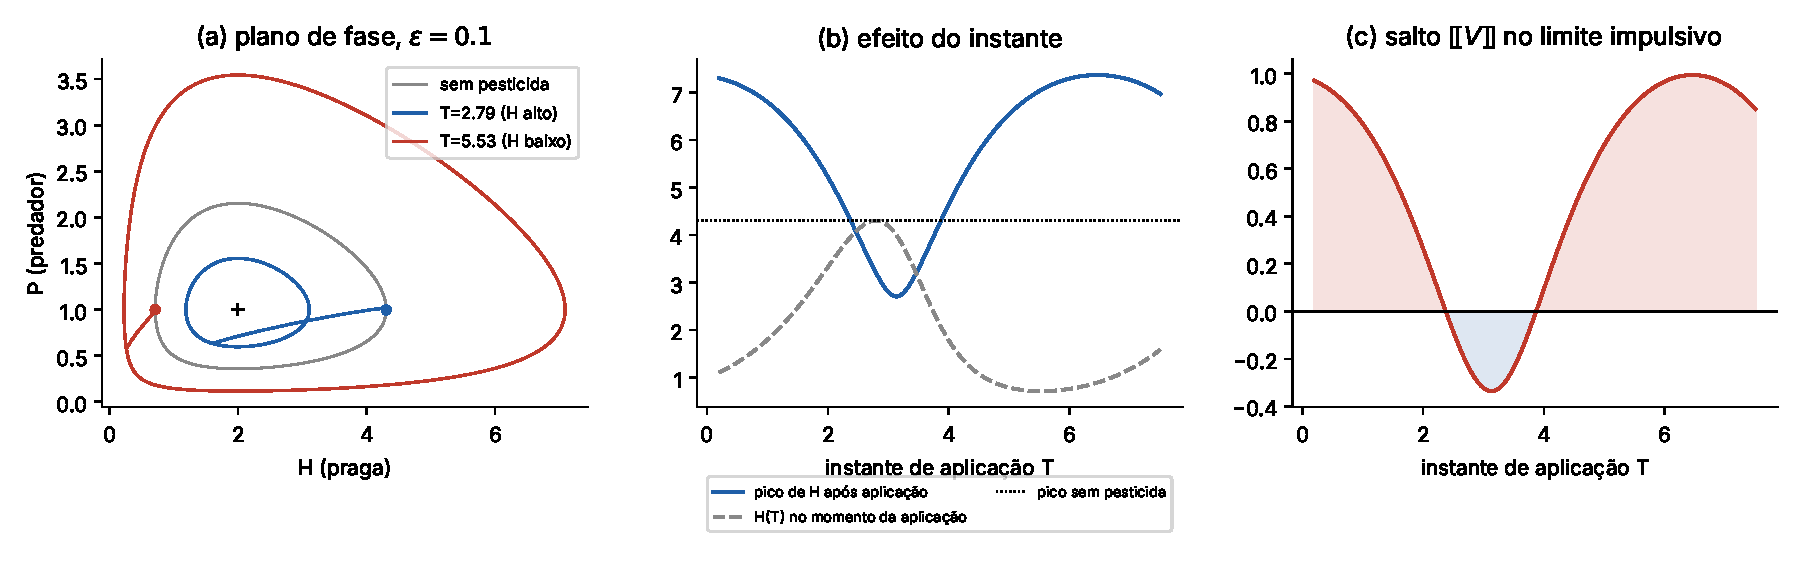
\includegraphics[width=\textwidth]{figuras/fig1_edo_instante.pdf}
\caption{Caso sem difusão, $s_H=1$, $s_P=0{,}5$, órbita inicial por $(1;0{,}5)$.
(a) Aplicar com $H$ alto ($T=2{,}79$) leva a um ciclo menor; aplicar com $H$ baixo
($T=5{,}53$) leva a um ciclo muito maior (ressurgência), ainda que o pesticida mate a praga.
(b) Pico futuro da praga em função do instante de aplicação. (c) Salto de energia
\eqref{eq:saltoE}: as regiões $\jump{V}>0$ coincidem com as de pico maior que o original,
como prevê a Proposição~\ref{prop:edo}.}
\label{fig:edo}
\end{figure}

\begin{figure}[ht]
\centering
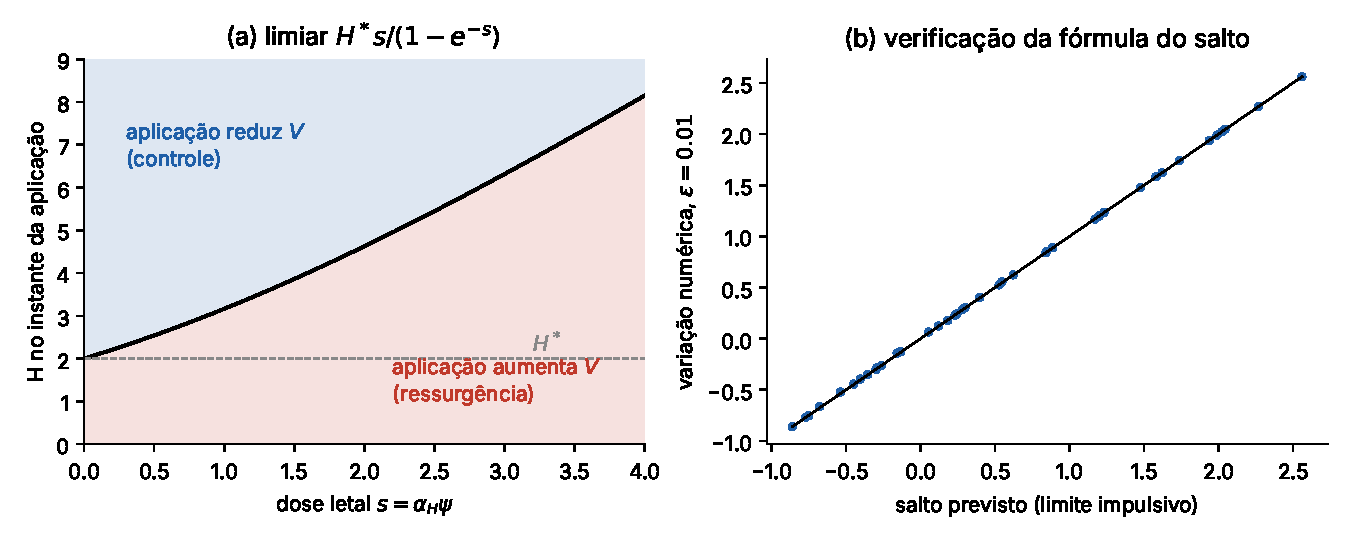
\includegraphics[width=0.85\textwidth]{figuras/fig2_limiar_dose.pdf}
\caption{(a) Limiar \eqref{eq:limiar} no plano (dose, população): acima da curva a aplicação
reduz a energia. (b) Verificação da fórmula do salto \eqref{eq:saltoE}: 40 estados e doses
aleatórios, pulso de duração $\epsilon=0{,}01$; erro máximo $0{,}016$, compatível com $O(\epsilon)$.}
\label{fig:limiar}
\end{figure}

\begin{figure}[ht]
\centering
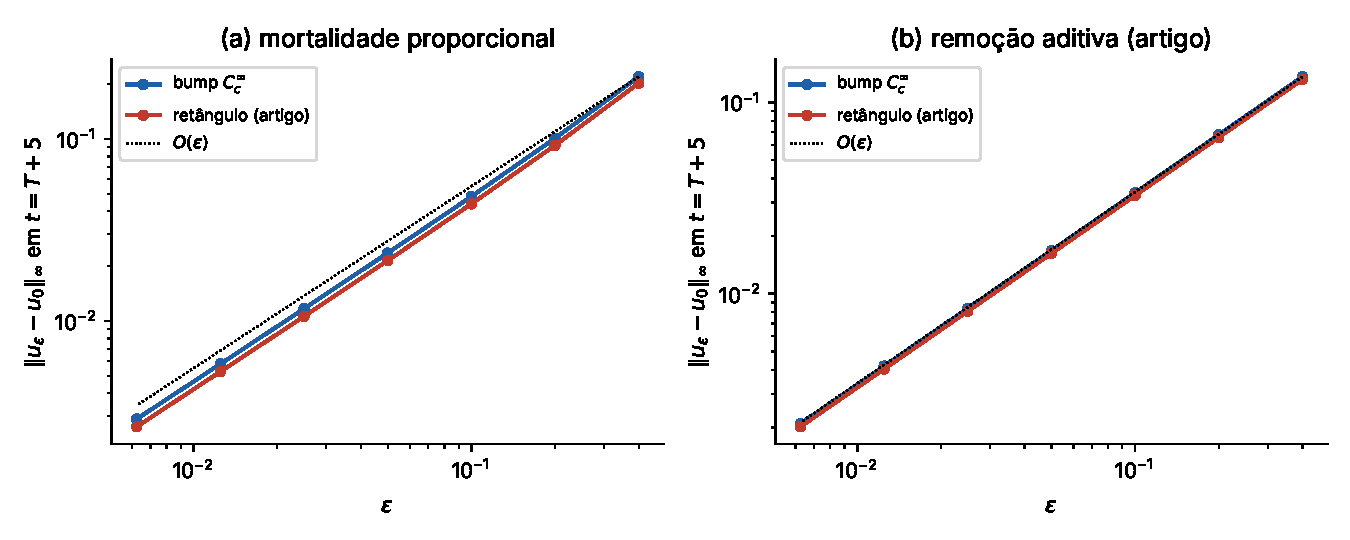
\includegraphics[width=0.85\textwidth]{figuras/fig3_convergencia.pdf}
\caption{Erro $\|u_\epsilon-u_0\|_\infty$ em $t=T+5$ (caso espacial, talhão de largura 6) em função
de $\epsilon$, para o pulso retangular de \cite{LiYang} e para o bump $C^\infty_c$. (a) Mortalidade
proporcional, $\alpha_H=1$, $\alpha_P=0{,}5$. (b) Remoção aditiva, $\alpha_H=1$, $\alpha_P=0{,}1$.
As ordens observadas são $1{,}00$--$1{,}13$ em todos os casos (Teorema~\ref{teo:limite} e
Observação~\ref{obs:ordem}).}
\label{fig:conv}
\end{figure}

\begin{table}[ht]
\centering\small
\setlength{\tabcolsep}{4pt}
\begin{tabular}{lccccccc}
\toprule
$\epsilon$ & $0{,}4$ & $0{,}2$ & $0{,}1$ & $0{,}05$ & $0{,}025$ & $0{,}0125$ & $0{,}00625$\\
\midrule
bump, proporcional & $2{,}19\mathrm{e}{-1}$ & $1{,}01\mathrm{e}{-1}$ & $4{,}82\mathrm{e}{-2}$ & $2{,}36\mathrm{e}{-2}$ & $1{,}17\mathrm{e}{-2}$ & $5{,}80\mathrm{e}{-3}$ & $2{,}89\mathrm{e}{-3}$\\
retângulo, proporcional & $2{,}02\mathrm{e}{-1}$ & $9{,}22\mathrm{e}{-2}$ & $4{,}39\mathrm{e}{-2}$ & $2{,}14\mathrm{e}{-2}$ & $1{,}06\mathrm{e}{-2}$ & $5{,}26\mathrm{e}{-3}$ & $2{,}62\mathrm{e}{-3}$\\
bump, aditivo & $1{,}36\mathrm{e}{-1}$ & $6{,}78\mathrm{e}{-2}$ & $3{,}37\mathrm{e}{-2}$ & $1{,}68\mathrm{e}{-2}$ & $8{,}39\mathrm{e}{-3}$ & $4{,}19\mathrm{e}{-3}$ & $2{,}09\mathrm{e}{-3}$\\
retângulo, aditivo & $1{,}32\mathrm{e}{-1}$ & $6{,}56\mathrm{e}{-2}$ & $3{,}26\mathrm{e}{-2}$ & $1{,}62\mathrm{e}{-2}$ & $8{,}10\mathrm{e}{-3}$ & $4{,}05\mathrm{e}{-3}$ & $2{,}02\mathrm{e}{-3}$\\
\bottomrule
\end{tabular}
\caption{Erros da Figura~\ref{fig:conv}.}
\end{table}

\begin{figure}[ht]
\centering
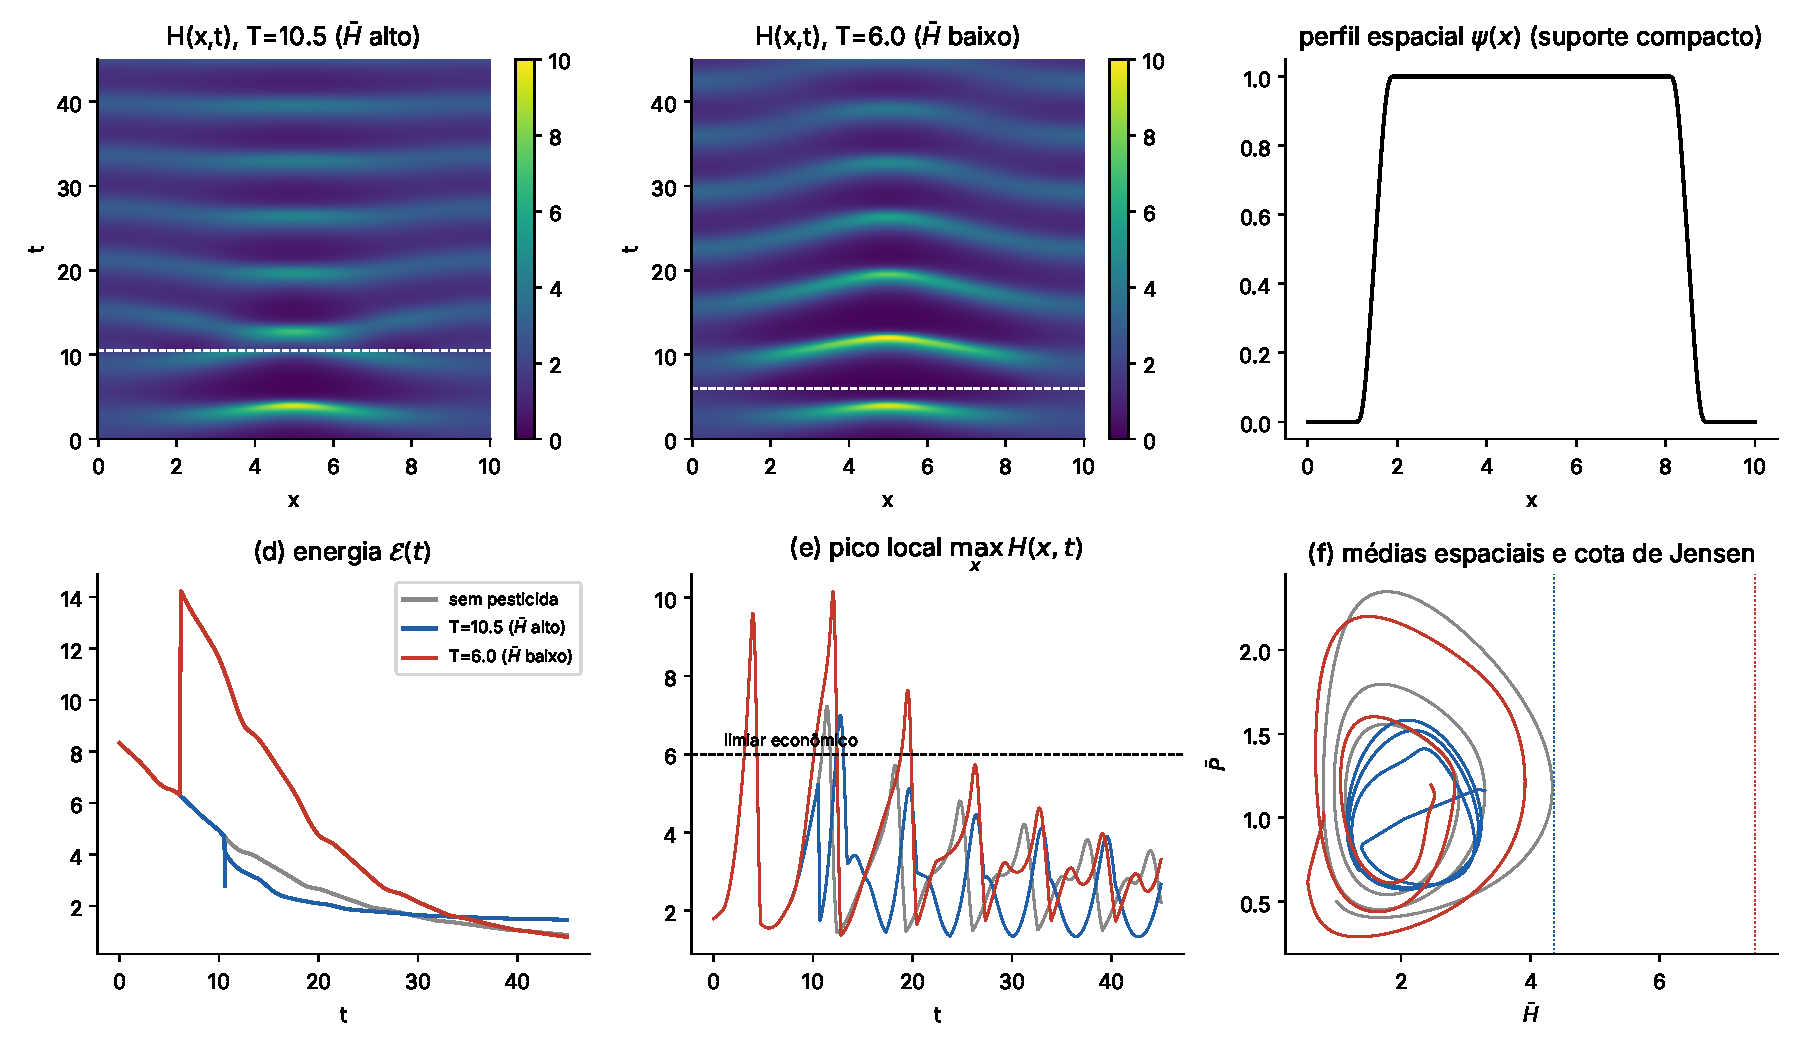
\includegraphics[width=\textwidth]{figuras/fig4_espacial.pdf}
\caption{Caso espacial, talhão $\psi$ de largura 8 (refúgios nas bordas), $s_H=1{,}2$, $s_P=0{,}6$,
$\epsilon=0{,}2$. Aplicação com média alta ($T=10{,}5$): $\E$ cai de $4{,}74$ para $4{,}02$ e o pico local
posterior é $6{,}99$ (contra $7{,}23$ sem pesticida). Aplicação com média baixa ($T=6$): $\E$ salta de
$6{,}34$ para $14{,}22$ e o pico local sobe para $10{,}16$, ultrapassando o limiar econômico
ilustrativo $6$ várias vezes. Em (d), observe que durante o pulso em $T=10{,}5$ a energia primeiro cai
e depois sobe (Corolário~\ref{cor:infinitesimal}). Em (f), as linhas pontilhadas são a cota
\eqref{eq:cota} para $\bar H$, respeitada pelas trajetórias das médias.}
\label{fig:espacial}
\end{figure}

\begin{figure}[ht]
\centering
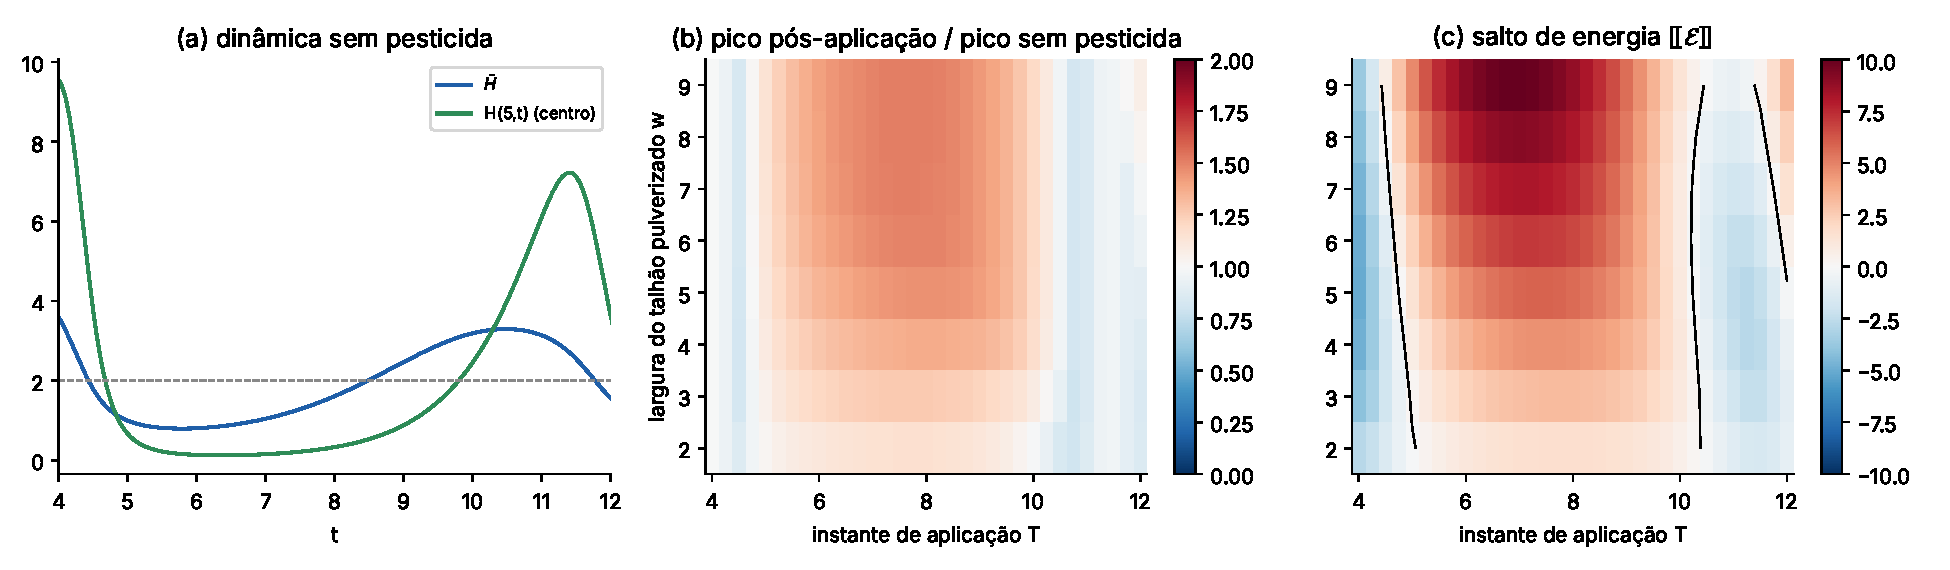
\includegraphics[width=\textwidth]{figuras/fig5_talhao.pdf}
\caption{Efeito conjunto do instante $T$ e da largura $w$ do talhão (centrado, refúgio nas bordas).
(a) Dinâmica sem pesticida: média e centro do domínio. (b) Razão entre o pico local de $H$ em
$[T,T+25]$ com e sem pesticida (vermelho: ressurgência). (c) Salto de energia; a curva preta é
$\jump{\E}=0$. As regiões de ressurgência em (b) praticamente coincidem com $\jump{\E}>0$ em (c). Talhões
estreitos (refúgio grande) atenuam tanto o benefício quanto o dano.}
\label{fig:talhao}
\end{figure}

\begin{figure}[ht]
\centering
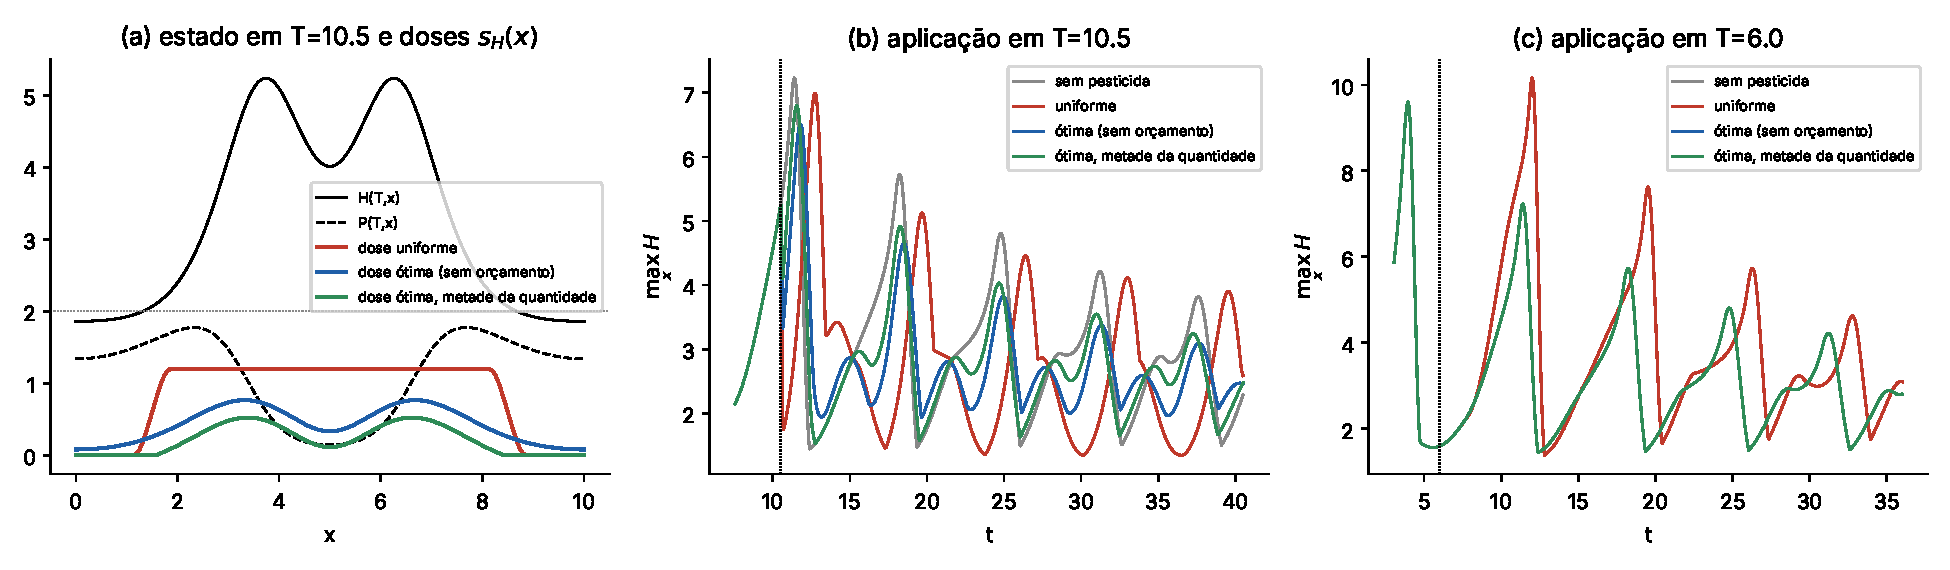
\includegraphics[width=\textwidth]{figuras/fig6_dose_otima.pdf}
\caption{Regra de dose ótima (Proposição~\ref{prop:otima}, $\kappa=0{,}5$). (a) Estado em $T=10{,}5$
e perfis de dose. (b) Em $T=10{,}5$: a dose uniforme (quantidade total $8{,}40$) dá
$\jump{\E}=-0{,}72$ e pico $6{,}99$; a dose ótima usa metade do produto ($4{,}27$) e dá
$\jump{\E}=-2{,}13$, pico $6{,}51$; com apenas $2{,}14$ ainda se obtém $\jump{\E}=-1{,}76$, pico $6{,}80$.
(c) Em $T=6$ a regra prescreve dose nula (não aplicar) e evita a ressurgência causada pela dose
uniforme ($\jump{\E}=+7{,}87$, pico $10{,}16$).}
\label{fig:otima}
\end{figure}

\clearpage
%======================================================================
\section{Discussão}

A troca de $\Delta_\epsilon$ por uma função de suporte compacto $\rho_\epsilon(t)\psi(x)$ tem três
efeitos. Matematicamente, garante o limite regular $\epsilon\to0$ (Teorema~\ref{teo:limite}): o
suporte compacto de $\psi$ em $\Omega$ preserva a condição de Neumann e a regularidade do dado
pós-salto. Biologicamente, permite modelar aplicações de duração finita e talhões com refúgio. E,
combinada com a mortalidade proporcional, preserva a positividade, que o termo aditivo original
não garante.

A identidade de energia \eqref{eq:identidade} é a ferramenta central. Ela mostra que difusão e
pesticida têm papéis distintos: a difusão sempre dissipa energia, enquanto o pesticida pode
injetá-la. As duas conclusões de \cite{LiYang} passam a ser enunciados precisos: uma aplicação é
benéfica, no sentido de reduzir $\E$ e portanto a cota \eqref{eq:cota}, se e somente se
$\int_\Omega\{c[H(1-e^{-s_H})-\Hs s_H]+[P(1-e^{-s_P})-\Ps s_P]\}>0$. Isso depende do instante
(via $H(T,\cdot)$, $P(T,\cdot)$), da dose (via $\theta(s)$) e do lugar (via $\psi$).

\begin{observacao}[termos de taxia]\label{obs:taxia}
O modelo (3.1)--(3.2) de \cite{LiYang} inclui os termos $\mp\partial_xP\,\partial_xH$
(perseguição e fuga). Eles acrescentam a \eqref{eq:identidade} a parcela
$\int_\Omega\partial_xH\,\partial_xP\,[c(1-\Hs/H)-(1-\Ps/P)]\dd x$, sem sinal definido. A análise
com taxia fica em aberto, assim como o caso de Dirichlet (fronteira hostil), em que $\ln H$ não é
integrável na fronteira.
\end{observacao}

\paragraph{Extensões naturais.} (1) Aplicações periódicas $T_k=k\tau$ e a análise de Floquet do
mapa de Poincaré impulsivo; (2) otimização conjunta de $(T_k,\psi_k)$ num horizonte finito, para a
qual \eqref{eq:saltoE} dá o gradiente instantâneo; (3) coeficientes espacialmente heterogêneos;
(4) modelos com resposta funcional de Holling, em que $V$ deixa de ser conservado e a energia deve
ser substituída por uma função de Lyapunov apropriada \cite{Hsu}.

%======================================================================
\begin{thebibliography}{99}
\bibitem{LiYang} Y.~C.~Li, Y.~Yang, On the paradox of pesticides,
\emph{Commun.\ Nonlinear Sci.\ Numer.\ Simul.} 29 (2015) 179--187.
\bibitem{Hardin} M.~Hardin, B.~Benrey, M.~Coll, W.~Lamp, G.~Roderick, P.~Barbosa,
Arthropod pest resurgence: an overview of potential mechanisms, \emph{Crop Prot.} 14 (1995) 3--18.
\bibitem{Lester} P.~Lester, H.~Thistlewood, R.~Harmsen, The effects of refuge size and number on
acarine predator--prey dynamics in a pesticide-disturbed apple orchard, \emph{J.\ Appl.\ Ecol.} 35
(1998) 323--331.
\bibitem{Heong} K.~Heong, A.~Manza, J.~Catindig, S.~Villareal, T.~Jacobsen, Changes in pesticide use
and arthropod biodiversity in the IRRI research farm, \emph{Outlooks Pest Manage.} 18 (2007) 229--233.
\bibitem{Henry} D.~Henry, \emph{Geometric Theory of Semilinear Parabolic Equations}, Lecture Notes in
Math.\ 840, Springer, 1981.
\bibitem{Pazy} A.~Pazy, \emph{Semigroups of Linear Operators and Applications to Partial Differential
Equations}, Springer, 1983.
\bibitem{ProtterWeinberger} M.~H.~Protter, H.~F.~Weinberger, \emph{Maximum Principles in Differential
Equations}, Prentice-Hall, 1967.
\bibitem{Hale} J.~K.~Hale, \emph{Asymptotic Behavior of Dissipative Systems}, AMS, 1988.
\bibitem{Hsu} S.-B.~Hsu, A survey of constructing Lyapunov functions for mathematical models in
population biology, \emph{Taiwanese J.\ Math.} 9 (2005) 151--173.
\bibitem{Lakshmikantham} V.~Lakshmikantham, D.~D.~Bainov, P.~S.~Simeonov, \emph{Theory of Impulsive
Differential Equations}, World Scientific, 1989.
\bibitem{Tang} S.~Tang, Y.~Xiao, L.~Chen, R.~A.~Cheke, Integrated pest management models and their
dynamical behaviour, \emph{Bull.\ Math.\ Biol.} 67 (2005) 115--135.
\bibitem{CantrellCosner} R.~S.~Cantrell, C.~Cosner, \emph{Spatial Ecology via Reaction--Diffusion
Equations}, Wiley, 2003.
\end{thebibliography}

\end{document}
